\subsection{Non-polar Solvation Free Energy Estimation}\label{subsec:CC_method}

The non-polar term in Equation \ref{eq:G_solv} can itself be decomposed into a sum of two free energies \cite{zacharias2003continuum}, $\Delta G_{cav}$ the creation of a solute-shaped cavity by turning on the potential short-range \textbf{repulsive interactions}, and $\Delta G_{disp}$, in which one turns on the longer-range \textbf{attractive} solute-solvent dispersion interactions.
\begin{equation}
    \Delta G_{np}=\Delta G_{cav} + \Delta G_{disp}
    \label{eq:G_np}
\end{equation}
Traditionally, $\Delta G_{cav}$ is highly correlated with the SASA factor previously described, however, the value of $\gamma$ does not agree with the surface tension coefficient and works as a adjustable parameter which can change the errors. On the other hand, $\Delta G_{disp}$ can be described with a continuum model, where the solute-solvent dispersion interaction potential is integrated over the solvent, which in turn can be formulated as an volume integral over the solvent accessible surface \cite{tan2007implicit}.
It is been study that while repulsive and attractive components of the non-polar part both scale roughly with surface area (or volume) of the solute, the total non-polar free energy does not scale with the solute surface area or volume. \cite{mobley2009small}.

\subsubsection{Implicit Solvent Model for $\Delta G_{cav}$ and $\Delta G_{disp}$}
A new approach to estimate $\Delta G_{cav}$ and $\Delta G_{disp}$ \cite{} proposes an implicit solvent model with a clearer physical meaning than current available models. Regarding Equations \ref{eq:G_solv} and \ref{eq:G_np}, the non-polar solvation free energy can be expressed as (See Figure \ref{fig:np_cycle}): 
\begin{equation}
    \Delta G_{solv}= \Delta G_{cav}+ \Delta G_{disp}+ \Delta G_{polar}
\end{equation}
\begin{figure}[h]
    \centering
    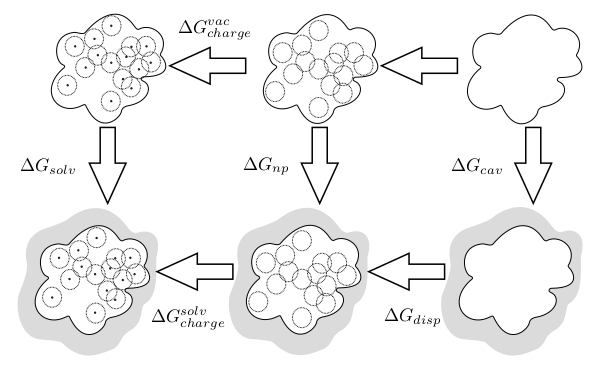
\includegraphics[scale=0.6]{Figures/Chapter 4/np_cycle.png}
    \caption{Thermodynamic cycle for solvation energy. Figure taken from \cite{cooper2020simple}}
    \label{fig:np_cycle}
\end{figure}

Using a capacitance-based approach for $\Delta G_{cav}$, the potential inside the solute is model as a constant $\phi_{static}$, defining the solute boundary as the solvent-excluded surface (SES) \cite{connolly1983analytical}. In the infinite solvent region, the potential is model as $\phi=0$, and bound the region using the boundary of the first solvation shell (the solvent-accessible surface, SAS \cite{connolly1983analytical}. These surfaces bound a shell, which is model as a macroscopic dielectric with the uniform relative permittivity $\epsilon_{shell}$, and where the electrostatic potential obeys the Laplace equation. Fixing the potentials at both boundaries implies that the dielectric constants of the solute and bulk solvent are irrelevant.. It is used $\epsilon_{shell}$ as a fitting parameter, but it has clear physical bounds and significance. The energy associated with this boundary-value problem can be solved using a pair of coupled boundary-integral equations for unknown charge densities on the two surfaces by: 
\begin{equation}
    \begin{bmatrix}
V_{diel} & V_{diel}\\ 
 V_{shell}& V_{shell}
\end{bmatrix}\begin{bmatrix}
\sigma_{diel}\\ 
\sigma_{shell}
\end{bmatrix}
=
\begin{bmatrix}
\phi_{static}\\ 
0
\end{bmatrix}
\end{equation}
where $V_{diel}(\phi_{shell})=\oint_{shell}\frac{\phi(r')}{4\pi\left |r_{diel}-r' \right |}$ denotes the potential induced at the inner surface (the dielectric boundary) by the surface charge distribution on the outer boundary (the solvent-accessible surface). Figure \ref{fig:capacitor} represent this idea. 
\begin{figure}[h]
    \centering
    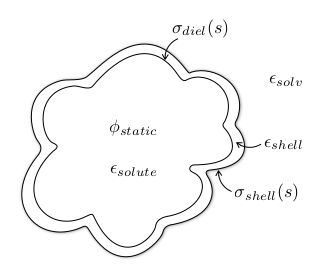
\includegraphics[scale=0.5]{Figures/Chapter 4/capacitor_model.png}
    \caption{Sketch of the capacitor model. Figure taken from \cite{cooper2020simple}}
    \label{fig:capacitor}
\end{figure}
Having found the surface charge distributions it is possible to compute the work (and hence, the free energy) required to charge the resulting capacitor with standard electrostatic theory
\begin{equation}
    \Delta G_{cav}=\int_{\Omega}\phi(r)\rho(r)dr
    \label{eq:g_cav}
\end{equation}
being $\rho$ the charge distribution, in this case, concentrated on the SAS ($\sigma_{shell}$) and SES ($\sigma_{diel}$)Noting that the potential on the outer surface is zero, we can rewrite Equation \ref{eq:g_cav} as: 
\begin{equation}
    \Delta G_{cav}=\oint_{diel}\phi_{static}\sigma_{diel}(r)dr
    \label{eq:int_shell}
\end{equation}

The previous $\Delta G_{cav}$ component is combine with a modification of a continuum integral method \cite{levy2003nonpolar} for calculating $\Delta G_{disp}$, by integrating the Lennard-Jones potential outside the solvent-accessible surface which can be formulated as a surface integral using the divergence theorem by: 
\begin{equation}
    \Delta G_{disp}=\sum_i \oint_{shell} \rho_w \frac{\partial}{\partial n}\left ( \frac{A_i}{90\left |r-r_i\right |^{10}} - \frac{B_i}{12\left |r-r_i\right |^{4}} \right )dr
    \label{eq:CC_implicit}
\end{equation}
where $\rho_w$ is considered to be the bulk number density, $A_i$ and $B_i$ re related to the Lennard-Jones parameters for the water oxygen and atom i, the sum is over the solute’s atoms, and the unit vector \textbf{n} points into the solvent.
Finally, a solvation-layer interface condition (SLIC) continuum electrostatics method   \cite{mehdizadeh2019solvation} is used to compute $\Delta G_{polar}$ (or $\Delta G_{charge}^{solv}$ in Figure \ref{fig:np_cycle}). (Notice that regarding the thermodynamic cycle represented in Figure \ref{fig:np_cycle},  $ \Delta G_{solv}$ is equivalent to $\Delta G_{charge}^{solv}$ - $\Delta G_{charge}^{vac}$).



 